\section{Polynomeilla laskeminen}

Polynomilausekkeiden käsittely on välttämätön taito matematiikassa, ja siksi tähän lukuun kannattaa paneutua huolella.

Polynomeja voidaan kertoa vakiolla kertomalla kukin termi erikseen.

\begin{esimerkki}
	Olkoon $P(x)=x^3-2x^2+1$. Määritä luvun $4P(3)$ arvo.
	\begin{esimratk}
	TAPA 1.
		Polynomi $P(x)$ kerrotaan vakiolla $4$ kertomalla kukin termi erikseen.
		\begin{align*}
		 4P(x)&=4(x^3-2x^2+1)\\
		 &=4x^3-4\cdot2x^2+4\cdot1\\
		 &=4x^3-8x^2+4.
		\end{align*}
		
		Määritetään polynomin $4P(x)$ arvo, kun $x=3$
		\begin{align*}
		 4P(3)&=4\cdot3^3-8\cdot3^2+4\\
			&=4\cdot27-8\cdot9+4\\
			&=108-72+4\\
			&=40.
		\end{align*}
	TAPA 2.
		Ratkaistaan ensin $P(3)$, ja kerrotaan se vasta sen jälkeen vakiolla $4$.
		\begin{align*}
		 P(3)&=3^3-2\cdot3^2+1\\
			&=27-2\cdot9+1\\
			&=27-18+1\\
			&=10,
		\end{align*}
		jolloin $4P(3)=4\cdot10=40$.
	\end{esimratk}
	\begin{esimvast}
	 $4P(3)=40$.
	\end{esimvast}
\end{esimerkki}


\subsection*{Polynomien yhteen- ja vähennyslasku}

\qrlinkki{http://opetus.tv/maa/maa2/polynomien-yhteen-ja-vahennyslasku/}
{Opetus.tv: \emph{polynomien yhteen- ja vähennyslasku} (7:36)}

Kaikkien polynomien summat ja erotukset ovat aina polynomeja. Polynomeja voidaan laskea yhteen yhdistämällä samanasteiset termit. On kätevää aloittaa ryhmittelemällä samanasteiset termit vierekkäin. Polynomit sievennetään yleensä aina yleiseen muotoon asti, jossa on vain yksi termi kutakin astetta kohti.

Samanasteisten termien yhteen- ja vähennyslasku perustuu siihen, että soveltamalla reaalilukujen osittelulakia $a(b\pm c)=ab\pm ac$ oikealta vasemmalle (ks. Vapaa matikka 1) samanasteiset potenssit voidaan ottaa yhteiseksi tekijäksi:

\[ ax^n \pm bx^n = (a \pm b)x^n \]

\begin{esimerkki}

	\begin{itemize}
	\item $2x+3x=(2+3)x=5x$
	\item $t-5t=1t-5t=(1-5)t=-4t$
	\item $5,1k^2+3,04k^2 = (5,1+3,04)k^2 = 8,14k^2$
	\item $\frac{1}{2}y^{42}+\frac{1}{3}y^{42}=(\frac{1}{2}+\frac{1}{3})y^{42}= (\frac{3}{6}+\frac{2}{6})y^{42}=\frac{3+2}{6}y^{42}=\frac{5}{6}y^{42}$
	\end{itemize}
\end{esimerkki}

\begin{esimerkki}
Laske polynomien $5x^2-x+5$ ja $3x^2-1$ summa.
    \begin{esimratk}
    
        \begin{align*}
            (\textcolor{blue}{5x^2} \textcolor{red}{{}-x} + 5) + (\textcolor{blue}{3x^2} -1) 
            &=\textcolor{blue}{5x^2} \textcolor{red}{{}-x} + 5 + \textcolor{blue}{3x^2} -1 \\
            &=\textcolor{blue}{5x^2+3x^2} \textcolor{red}{{}-x} +5-1\\
%                       &=\textcolor{blue}{(5+3)x^2} \textcolor{red}{{}-x}+(5-1)\\
            &=\textcolor{blue}{8x^2} \textcolor{red}{{}-x}+4.
        \end{align*}     
    \end{esimratk}
    \begin{esimvast}
        Polynomien summa on $8x^2-x+4$.
    \end{esimvast}
\end{esimerkki}

Edellisessä esimerkissä molemmat yhteenlaskettavat polynomit laitettiin rakenteen selventämisen vuoksi kaarisulkeiden sisään, vaikka niillä ei ollutkaan laskujärjestyksen kannalta mitään merkitystä.

Polynomeja voidaan vastaavalla tavalla vähentää toisistaan. Vähennyslaskun tapauksessa on tärkeää laittaa vähennettävä polynomi sulkeisiin, sillä miinusmerkki vaikuttaa \emph{koko} polynomiin, ei vain sen ensimmäiseen termiin. Sulkeet avattaessa pitää muistaa vaihtaa kaikkien termien merkki: 

\begin{esimerkki}
    Laske polynomien $4x^3+1$ ja $6x^3-2$ erotus.
    \begin{esimratk}
        \begin{align*}
		(\textcolor{blue}{4x^3}+1)-(\textcolor{blue}{6x^3}-2) \\
		&= \textcolor{blue}{4x^3}+1 - \textcolor{blue}{6x^3} -(-2) \\
		&= \textcolor{blue}{4x^3}+1 - \textcolor{blue}{6x^3} + 2 \\
		&= \textcolor{blue}{4x^3-6x^3} +1 +2 \\
		&=\textcolor{blue}{-2x^3}+3
        \end{align*}
    \end{esimratk}
    \begin{esimvast}
        Polynomien erotus on $-2x^3+3$.
    \end{esimvast}
\end{esimerkki}

\begin{esimerkki}
    Laske polynomien $14x^3+69$ ja $3x^3+2x^2+x$ erotus.
    \begin{esimratk}
        \begin{align*}
            (\textcolor{blue!30!green}{14x^3} + 69) - (\textcolor{blue!30!green}{3x^3} \textcolor{blue}{{}+ 2x^2} \textcolor{red}{{}+x})
            &= \textcolor{blue!30!green}{14x^3} + 69 \textcolor{blue!30!green}{{}-3x^3} \textcolor{blue}{-2x^2} \textcolor{red}{{}-x} \\
            &= \textcolor{blue!30!green}{14x^3{}-3x^3} \textcolor{blue}{{}-2x^2} \textcolor{red}{{}-x} + 69 \\
%           &= \textcolor{blue!30!green}{(14{}-3)x^3} \textcolor{blue}{{}-2x^2} \textcolor{red}{{}-x} + 69 \\
            &= \textcolor{blue!30!green}{11x^3} \textcolor{blue}{{}-2x^2} \textcolor{red}{{}-x} + 69
        \end{align*}
    \end{esimratk}
    \begin{esimvast}
        Polynomien erotus on $11x^3-2x^2-x+69$.
    \end{esimvast}
\end{esimerkki}

\begin{esimerkki}
    Olkoot polynomit $P(x)=2x+1$ ja $Q(x)=3x^2-2x+5$. Määritä summa $R(x)=P(x)+Q(x)$.
    \begin{esimratk}
        \begin{align*}
            R(x) = P(x)+Q(x) &= (2x+1)+(3x^2-2x+5) \\
                             &= 2x+1+3x^2-2x+5 \\
                             &= 3x^2+2x-2x+1+5 \\
                             &= 3x^2+6.
        \end{align*}
    \end{esimratk}
    \begin{esimvast}
        $R(x) = 3x^2+6$.
    \end{esimvast}
\end{esimerkki}

\begin{esimerkki}
    Laske polynomien $P$ ja $Q$ erotus $R$, kun $P(x)=-3x^4+x^2+1$ ja $Q(x)=-3x^4+3x^3-x$.
    Mikä on polynomin $R$ aste?
   \begin{esimratk}
        \begin{align*}
            R(x) = P(x)-Q(x) &= (-3x^4+x^2+1)-(-3x^4+3x^3-x) \\
                             &= -3x^4+x^2+1+3x^4-3x^3+x \\
                             &= -3x^4+3x^4-3x^3+x^2+x+1 \\
                             &= -3x^3+x^2+x+1.
        \end{align*}
    \end{esimratk}
    \begin{esimvast}
        $R(x) = -3x^3+x^2+x+1$. Polynomin $R$ aste on kolme.
    \end{esimvast}
\end{esimerkki}

\subsection*{Polynomien kertolasku}

\qrlinkki{http://opetus.tv/maa/maa2/polynomien-kertolasku/}
{Opetus.tv: \emph{polynomien kertolasku} (10:00)}

\subsubsection*{Monomien tulo}

Kahden monomin tulo sievennetään kertomalla kertoimet keskenään ja kirjainosat keskenään. Muista potenssien laskusäännöt (ks. Vapaa matikka 1)!

\begin{esimerkki}
    Laske \quad 
    a) $2x\cdot 3x$ \quad
    b)$-3x^2\cdot (-5x^4)$ \quad
    c) $5x^2 \cdot (-2x)$
    \begin{esimratk}
        \begin{alakohdat}
            \alakohta{$2x\cdot 3x = 2\cdot 3\cdot x\cdot x = 6x^2$}
            \alakohta{$-3x^2\cdot (-5x^4) = (-3)\cdot (-5) \cdot x^2 \cdot x^4 = 15 x^6$}
            \alakohta{$5x^2 \cdot (-2x) = -10 x^3$}
        \end{alakohdat}
    \end{esimratk}
    \begin{esimvast}
        a) $6x^2$ \quad
        b) $15x^6$ \quad
        c) $-10x^3$
    \end{esimvast}
\end{esimerkki}

\subsubsection*{Polynomin kertominen monomilla}

Polynomeja voi kertoa keskenään reaalilukujen tuttujen laskusääntöjen avulla. Yksinkertaisin erikoistapaus on polynomin kertominen monomilla, jolloin
käytetään osittelulakia $a(b+c)=ab+ac$.

\begin{esimerkki}
Laske \quad a) $5\cdot(x+3)$ \quad b) $2x(x-5)$ \quad 
c) $3(a+b+c)$
\begin{alakohdat}
    \alakohta{$5\cdot(x+3) = 5\cdot x + 5\cdot 3 = 5x+15$}
    \alakohta{$2x(x-5)=2x\cdot x -2\cdot x \cdot 5 = 2x^2-10x$}
    \alakohta{$3(a+b+c)=3a+3b+3c$}
\end{alakohdat}
\end{esimerkki} 

\subsubsection*{Kahden binomin tulo}

Kahden binomin tulon laskusääntö perustellaan soveltamalla osittelulakia kahdesti:

\begin{align*}
(a+b)(c+d) &= (a+b)\cdot c + (a+b)\cdot d &\emph{osittelulaki} \\
 &= ac+bc+ad+bd &\emph{osittelulaki} 
\end{align*}

Kahden binomin tulossa siis kummallakin ensimmäisen binomin termillä kerrotaan toisen binomin termit. Saadut neljä tuloa lasketaan yhteen. 

\newcommand{\pbezier}[4]{
	\pgfmathsetmacro{\PBxa}{#1}
	\pgfmathsetmacro{\PBxb}{#2}
	\pgfmathsetmacro{\PBya}{#3}
	\pgfmathsetmacro{\PByb}{#3+#4}
	\pgfmathsetmacro{\PBca}{0.8 * \PBxa + 0.2 * \PBxb}
	\pgfmathsetmacro{\PBcb}{0.2 * \PBxa + 0.8 * \PBxb}
	\draw[color=red] (\PBxa, \PBya) .. controls (\PBca, \PByb) and (\PBcb, \PByb) .. (\PBxb, \PBya);
}

\begin{esimerkki}
Laske binomien $x+2$ ja $x-5$ tulo. \\
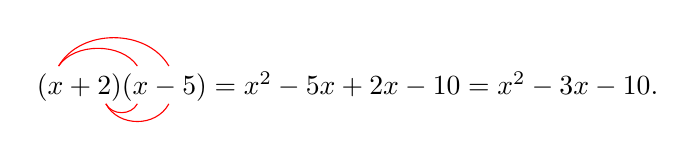
\begin{tikzpicture}
\draw node[right] {$(x+2)(x-5) = x^2-5x+2x-10 = x^2 -3x-10.$};

\pgfmathsetmacro{\klAx}{0.40}
\pgfmathsetmacro{\klBx}{1.00}
\pgfmathsetmacro{\klCx}{1.4}
\pgfmathsetmacro{\klDx}{1.8} 
\pgfmathsetmacro{\klEx}{2.5}
\pgfmathsetmacro{\klLo}{-0.22}
\pgfmathsetmacro{\klHi}{0.26}

\pbezier{\klAx}{\klCx}{\klHi}{0.3}
\pbezier{\klAx}{\klDx}{\klHi}{0.48}

\pbezier{\klBx}{\klCx}{\klLo}{-0.15}
\pbezier{\klBx}{\klDx}{\klLo}{-0.3}
\end{tikzpicture}\newline
\end{esimerkki}

\begin{esimerkki}
Laske binomien $x^2-x$ ja $2x-1$ tulo. \\
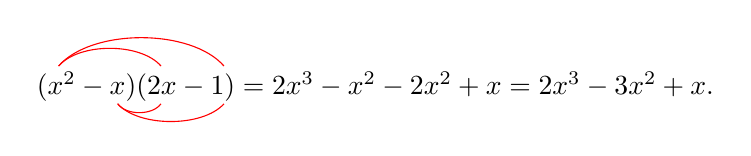
\begin{tikzpicture}
\draw node[right] {$(x^2-x)(2x-1) = 2x^3-x^2-2x^2+x = 2x^3 -3x^2 +x.$};

\pgfmathsetmacro{\klAx}{0.40}
\pgfmathsetmacro{\klBx}{1.15}
\pgfmathsetmacro{\klCx}{1.7}
\pgfmathsetmacro{\klDx}{2.5}
\pgfmathsetmacro{\klEx}{2.7}
\pgfmathsetmacro{\klLo}{-0.22}
\pgfmathsetmacro{\klHi}{0.26}

\pbezier{\klAx}{\klCx}{\klHi}{0.3}
\pbezier{\klAx}{\klDx}{\klHi}{0.48}

\pbezier{\klBx}{\klCx}{\klLo}{-0.15}
\pbezier{\klBx}{\klDx}{\klLo}{-0.3}
\end{tikzpicture}\newline
\end{esimerkki}




\subsubsection*{Yleinen kertolasku}

Osittelulain nojalla kahden polynomin tulo saadaan laskemalla yhteen kaikki
termit, jotka saadaan kertomalla termi ensimmäisestä ja toinen termi toisesta
polynomista.


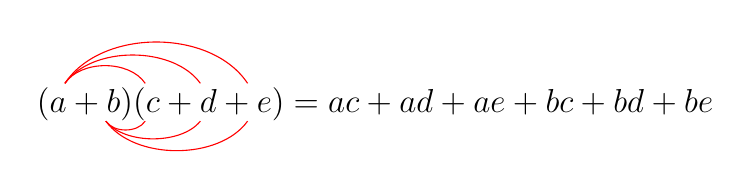
\begin{tikzpicture}
\draw node[right] {\large $(a+b)(c+d+e) = ac+ad+ae+bc+bd+be$};

\pgfmathsetmacro{\klAx}{0.48}
\pgfmathsetmacro{\klBx}{1.0}
\pgfmathsetmacro{\klCx}{1.5}
\pgfmathsetmacro{\klDx}{2.2}
\pgfmathsetmacro{\klEx}{2.8} %oli 3.26
\pgfmathsetmacro{\klLo}{-0.22}
\pgfmathsetmacro{\klHi}{0.26}

\pbezier{\klAx}{\klCx}{\klHi}{0.3}
\pbezier{\klAx}{\klDx}{\klHi}{0.48}
\pbezier{\klAx}{\klEx}{\klHi}{0.7}

\pbezier{\klBx}{\klCx}{\klLo}{-0.15}
\pbezier{\klBx}{\klDx}{\klLo}{-0.3}
\pbezier{\klBx}{\klEx}{\klLo}{-0.5}
\end{tikzpicture}

\begin{esimerkki}
Laske polynomien $x-3$ ja $x^2-4x+3$ tulo. \\
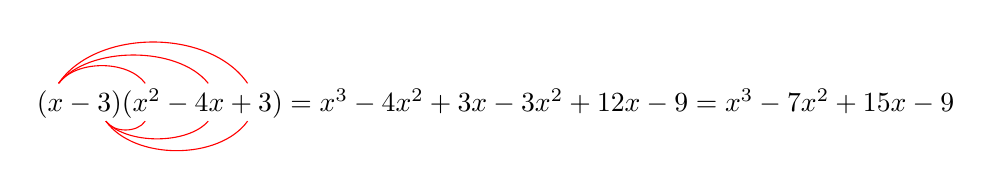
\begin{tikzpicture}
\draw node[right] {$(x-3)(x^2-4x+3) = x^3-4x^2+3x-3x^2+12x-9 = x^3-7x^2+15x-9$};

\pgfmathsetmacro{\klAx}{0.40}
\pgfmathsetmacro{\klBx}{1.00}
\pgfmathsetmacro{\klCx}{1.5}
\pgfmathsetmacro{\klDx}{2.3}
\pgfmathsetmacro{\klEx}{2.8}
\pgfmathsetmacro{\klLo}{-0.22}
\pgfmathsetmacro{\klHi}{0.26}

\pbezier{\klAx}{\klCx}{\klHi}{0.3}
\pbezier{\klAx}{\klDx}{\klHi}{0.48}
\pbezier{\klAx}{\klEx}{\klHi}{0.7}

\pbezier{\klBx}{\klCx}{\klLo}{-0.15}
\pbezier{\klBx}{\klDx}{\klLo}{-0.3}
\pbezier{\klBx}{\klEx}{\klLo}{-0.5}
\end{tikzpicture}\newline
\end{esimerkki}

\begin{esimerkki}
Laske polynomien $x^4-3x^3+3$ ja $x^3-2x^2+1$ tulo. \\
\begin{align*}
&\hspace{0.5cm}(\textcolor{red}{x^4} \textcolor{blue}{-3x^3} +{}\textcolor{blue!30!green}{3})(x^3-2x^2+1) \\
&= \textcolor{red}{x^4}\cdot x^3 + \textcolor{red}{x^4}\cdot (-2x^2)+\textcolor{red}{x^4}\cdot 1\textcolor{blue}{{}-3x^3}\cdot x^3\textcolor{blue}{{}-3x^3}\cdot(-2x^2)\textcolor{blue}{{}-3x^3}\cdot1 \\
&\hspace{0.5cm}+\textcolor{blue!30!green}{3}x^3+\textcolor{blue!30!green}{3}\cdot(-2x^2)+\textcolor{blue!30!green}{3}\cdot 1 \\
&= x^7-2x^6+x^4-3x^6+6x^5-3x^3+3x^3-6x^2+3 \\
&= x^7-5x^6+6x^5+x^4-6x^2+3
\end{align*}
\end{esimerkki}

\begin{tehtavasivu}

\paragraph*{Opi perusteet}

\begin{tehtava}
    Sievennä.
    \begin{enumerate}[a)]
        \item $3x+5x $
        \item $4x^2+7x^2$
        \item $-6y+2y $
        \item $3x-(-2x)$
    \end{enumerate}
    \begin{vastaus}
        \begin{enumerate}[a)]
            \item $8x$
            \item $11x^2$
            \item $-4y$
            \item $5x$
        \end{enumerate}
    \end{vastaus}
\end{tehtava}

\begin{tehtava}
    Sievennä.
    \begin{enumerate}[a)]
    	\item $5x-2+2x+7$
        \item $5x-3y-y-2x$
        \item $2x^2+x+x^2-5x$
        \item $y^3 - 2y^2+4y^3-y $
    \end{enumerate}
    \begin{vastaus}
        \begin{enumerate}[a)]
        	\item $7x+5$
            \item $3x-4y$
            \item $3x^2-4x$
            \item $5y^3-2y^2-y$
        \end{enumerate}
    \end{vastaus}
\end{tehtava}

\begin{tehtava}
    Sievennä.
    \begin{enumerate}[a)]
        \item $(x^2 - 2x + 1) + (-x^2 + x) $
        \item $(3y^3 + 2y^2  + y) - (-y^2 + y)$
        \item $(z^{10} - z^6 + z^2 + 1) + (z^{10} + 2z^8 - 3z^6)$
    \end{enumerate}
    \begin{vastaus}
        \begin{enumerate}[a)]
            \item $-x + 1$
            \item $3y^3 + 3y^2$
            \item $2z^{10} + 2z^8 - 4z^6 + z^2 + 1$
        \end{enumerate}
    \end{vastaus}
\end{tehtava}

\begin{tehtava}
    Olkoot $P(x)=x^2+3x+4$ ja $Q(x)=x^3-10x+1$. Sievennä
    \begin{enumerate}[a)]
        \item $P(x)+Q(x)$
        \item $P(x)-Q(x)$
        \item $Q(x)-P(x)$
        \item $2P(3)+Q(2)$.
    \end{enumerate}
    \begin{vastaus}
        \begin{enumerate}[a)]
            \item $x^3+x^2-7x+5$ % x^2+3x+4 + x^3-10x+1
            \item $-x^3+x^2+13x+3$ % x^2+3x+4 -(x^3-10x+1) = x^2+3x+4 -x^3+10x-1
            \item $x^3-x^2-13x-3$ % 
            \item $33$ % 2*(3^2+3*3+4) +  2^3-10*2+1 = 2*(9+9+4)+8-20+1 =44-11 =33
        \end{enumerate}
    \end{vastaus}
\end{tehtava}

\begin{tehtava}
	Sievennä polynomifunktiot ja laske funktioiden arvot muuttujan arvoilla $1$, $-1$ ja $3$.
	\begin{enumerate}[a)]
		\item $P(x)=(x^3-4x+5)+(-x^3+x^2+4x-2)$
		\item $Q(x)=(2x^3+x^2-10x)-(3x^3-4x^2+5x)$
	\end{enumerate}
	
	\begin{vastaus}
		\begin{enumerate}[a)]
			\item $P(x)=x^2+3$, $P(1)=4$, $P(-1)=4$ ja $P(3)=12$
			\item $Q(x)=-x^3+5x^2-15x$, $Q(1)=21$, $Q(-1)=-9$ ja $R(3)=-27$
		\end{enumerate}
	\end{vastaus}
\end{tehtava}

\begin{tehtava}
     Sievennä
     \begin{enumerate}[a)]
         \item $(2x + 3) + x $
         \item $(3x - 1) + (-x + 1)$
         \item $(5x + 10) + (6x - 6) - (x + 3)$
     \end{enumerate}
     \begin{vastaus}
         \begin{enumerate}
             \item $3x + 3$
             \item $2x$
             \item $10x + 1$
         \end{enumerate}
     \end{vastaus}
 \end{tehtava}

\begin{tehtava}
	Sievennä polynomifunktiot ja laske funktioiden arvot muuttujan arvoilla $1$, $-1$ ja $3$.
	\begin{enumerate}[a)]
		\item $R(x)=4(2x-4)+(-x^3+1)$
		\item $S(x)=-(2x^2-x+8)+6(x^5-3x^2+1)$ \\ $-2(3x^5-10x^2)$
	\end{enumerate}
	\begin{vastaus}
		\begin{enumerate}[a)]
			\item $R(x)=-x^3+8x-15$, $R(1)=-8$, $R(-1)=-22$ ja $R(3)=-18$
			\item $S(x)=-2$, $S(1)=-1$, $S(-1)=-3$ ja $S(3)=1$
		\end{enumerate}
	\end{vastaus}
\end{tehtava}

\begin{tehtava}
    Sievennä.
    \begin{alakohdat}
        \alakohta{$x\cdot x^2$}
        \alakohta{$5x\cdot 3x$}
        \alakohta{$-2(-5x^3)$}
        \alakohta{$3x^2\cdot(-6x^4)$}
    \end{alakohdat}
    \begin{vastaus}
        \begin{alakohdat}
            \alakohta{$x^3$}
            \alakohta{$15x^2$}
            \alakohta{$10x^3$}
            \alakohta{$-18x^6$}
        \end{alakohdat}
    \end{vastaus}
\end{tehtava}

\begin{tehtava}
    Sievennä.
    \begin{alakohdat}
        \alakohta{$2(x+3)$}
        \alakohta{$x(x - 2)$}
        \alakohta{$3x(1-2x)$}
        \alakohta{$x^2(x + 5)$}
    \end{alakohdat}
    \begin{vastaus}
        \begin{alakohdat}
            \alakohta{$2x+6$}
            \alakohta{$x^2 - 2x$}
            \alakohta{$3x-6x^2$}
            \alakohta{$x^3 + 5x^2$}
        \end{alakohdat}
    \end{vastaus}
\end{tehtava}

\begin{tehtava}
    Sievennä.
    \begin{alakohdat}
        \alakohta{$3(x+2y-4)$}
        \alakohta{$(x+2)(x + 3)$}
        \alakohta{$(3-x)(2x-1)$}
\end{alakohdat}
    \begin{vastaus}
        \begin{alakohdat}
            \alakohta{$3x+6y-12$}
            \alakohta{$x^2 +5x+6$}
            \alakohta{$-2x^2+7x-3$}
        \end{alakohdat}
    \end{vastaus}
\end{tehtava}

\begin{tehtava}
    Sievennä lauseke $(x^2+1)(x^3-2x)$. Mikä on polynomin aste?
    \begin{vastaus}
        Lauseke sievenee muotoon $x^5-x^3-2x$. Polynomin aste on $5$.
    \end{vastaus}
\end{tehtava}

\paragraph*{Hallitse kokonaisuus}

\begin{tehtava}
	Mitkä seuraavista polynomilausekkeista esittävät samaa polynomifunktiota kuin
	$x^3+2x+1$?
	\begin{enumerate}[a)]
		\item $2x+x^3+1$
		\item $x^2+2x+1$
		\item $x+2x^3+1 - (x^3+x)$
		\item $15+x^4+2x+x^3-x^4-14$
	\end{enumerate}
	\begin{vastaus}
		a) ja d)
	\end{vastaus}
\end{tehtava}

\begin{tehtava}
	Mitkä ovat seuraavien polynomifunktioiden asteet, ts. sievennettyjen muotojen asteet?
	\begin{enumerate}[a)]
		\item $x+5-x$
		\item $x^2+x-2x^2$
		\item $4x^5+x^2-4-x^2$
		\item $x^4-2x^3+x-1+x^3-x^4+x^3$
	\end{enumerate}

	\begin{vastaus}
		\begin{enumerate}[a)]
			\item $0$
			\item $2$
			\item $5$
			\item $1$
		\end{enumerate}
	\end{vastaus}
\end{tehtava}

\begin{tehtava}
    Pohdi ja määritä sulkuja avaamatta lausekkeen $(x^2+1)(x^3-2x)$
    \begin{alakohdat}
        \alakohta{aste}
        \alakohta{vakiotermi.}
    \end{alakohdat}
    \begin{vastaus}
        \begin{alakohdat}
            \alakohta{Polynomin aste on kunkin tekijän korkeimpien asteiden summa, tässä siis $2+3=5$.}
            \alakohta{Polynomin vakiotermi on kunkin tekijän vakiotermien tulo, tässä siis $1\cdot 0=0$.}
        \end{alakohdat}
    \end{vastaus}
\end{tehtava}

\begin{tehtava}
    Sievennä.
    \begin{alakohdat}
        \alakohta{$(-2x)(4x - 1)\cdot 3$}
        \alakohta{$(-x^3)(10x - 2)$}
        \alakohta{$5(-2x + 1)(-9x) $}
        \alakohta{$2x(x-3)+1$}
    \end{alakohdat}
    \begin{vastaus}
        \begin{alakohdat}
            \alakohta{$-24x^2 + 6x$}
            \alakohta{$-10x^4 + 2x^3$}
            \alakohta{$90x^2 - 45x$}
            \alakohta{$2x^2-6x+1$}
        \end{alakohdat}
    \end{vastaus}
\end{tehtava}


\begin{tehtava}
    Sievennä.
    \begin{alakohdat}
        \alakohta{$(2y+5)(y+7)$}
        \alakohta{$(x-1)(x+4)x$}
    \end{alakohdat}
    \begin{vastaus}
        \begin{alakohdat}
            \alakohta{$2y^2 + 19y + 35$}
            \alakohta{$x^3 + 3x^2 - 4x$}
        \end{alakohdat}
    \end{vastaus}
\end{tehtava}


\begin{tehtava}
Ensimmäisen asteen polynomiausekkeen yleinen muoto on $ax+b$, missä $x$ on muuttuja, ja $a$ ja $b$ ovat (reaalisia) vakioita. Osoita, että jos $P$ ja $Q$ ovat ensimmäisen asteen polynomifunktioita, niin tällöin $P(Q(x))$ ja $Q(P(x))$ ovat myös ensimmäistä astetta.

	\begin{vastaus}
Voidaan merkitään $P(x)=ax+b$ ja $Q(x)=cx+d$, koska molemmat funktiot ovat ensimmäisen asteen polynomifunktioita. (Käytämme kertoimien merkitsemiseen eri kirjaimia, sillä lausekkeiden vakiot saattavat olla keskenään erisuuret.) Sievennetään $P(Q(x))$: $P(Q(x))=P(cx+d)=a(cx+d)+b=acx+ad+b$. Todetaan, että jos $a$ ja $c$ ovat reaalilukuvakioita, niin myös niiden tulo on reaalilukuvakio. Sama pätee vakioille $a$ ja $d$, joiden tulo ja myös kyseisen tulon ja $b$:n summa on vakio. Merkitään havainnollistamisen vuoksi $ac=e$, ja $ad+b=f$. Nyt lauseke $acx+ad+b$ voidaan kirjoittaa uudelleen muodossa $ex+f$, josta nähdään selvästi kyseessä olevan ensimmäisen asteen polynomi.

Väite osoitetaan järjestykselle $Q(P(x))$ samalla tavalla, minkä jälkeen väite on todistettu.

	\end{vastaus}
\end{tehtava}

\paragraph*{Lisää tehtäviä}

\begin{tehtava}
	Sievennä. 
	\begin{alakohdat}
		\alakohta{$(x-3)(2x^3-3x+4)$}
		\alakohta{$(x^2+1)(x^3-2x-4)$}
		\alakohta{$(x-1)(x^4+x^3+x^2+x+1)$}
		\alakohta{$(\frac{x}{5}-\frac{2}{3})(x^2+x+1)$}  %TÄMÄ TÄYTYY TARKISTAA
	\end{alakohdat}
	\begin{vastaus}
		\begin{alakohdat}
			\alakohta{$2x^4-6x^3-3x^2+13x-12$}
			\alakohta{$x^5-x^3-4x^2-2x-4$}
			\alakohta{$x^5-1$}
			\alakohta{$\frac{1}{5}x^3-\frac{7}{15}x^2-\frac{7}{15}x-\frac{2}{3}$}
		\end{alakohdat}
	\end{vastaus}
\end{tehtava}

	\begin{tehtava}
Sievennä $\sqrt{\frac{(a+b)^2 + (a-b)^2}{a^2 + b^2}}$.
	\begin{vastaus}
$\sqrt{2}$
	\end{vastaus}
	\end{tehtava}

\begin{tehtava}
    Olkoon $P(x)=-x^4+2x$ reaalifunktio. Sievennä lausekkeet.
    \begin{alakohdat}
		\alakohta{$P(\sqrt{2})$}
        \alakohta{$P(x)^2$}
        \alakohta{$P(-x)$}
        \alakohta{$P(2t)$}
    \end{alakohdat}
    \begin{vastaus}
        \begin{alakohdat}
            \alakohta{$-4 + 2\sqrt{2}$}
            \alakohta{$x^8 - 4x^5 + 4x^2$}
            \alakohta{$-x^4-2x$}
            \alakohta{$-16t^4+4t$}
        \end{alakohdat}
    \end{vastaus}
\end{tehtava}

\begin{tehtava}
    Olkoot $P(x)=x^2$ ja $Q(x)=x+1$ reaalifunktioita. Sievennä lausekkeet.
    \begin{alakohdat}
        \alakohta{$P(x+1)$}
        \alakohta{$Q(x-1)$}
        \alakohta{$P(Q(x))$}
        \alakohta{$Q(P(x))$}
    \end{alakohdat}
    \begin{vastaus}
        \begin{alakohdat}
            \alakohta{$P(x+1) = (x+1)^2 = x^2+2x+1$}
            \alakohta{$Q(x-1) = (x-1)+1 = x$}
            \alakohta{$P(Q(x)) = P(x+1) = (x+1)^2 = x^2+2x+1$}
            \alakohta{$Q(P(x)) = Q(x^2) = x^2+1$}
        \end{alakohdat}
    \end{vastaus}
\end{tehtava}

\end{tehtavasivu}